%%%%%%%%%%%%%%%%%%%%%%%%%%%%% Define Article %%%%%%%%%%%%%%%%%%%%%%%%%%%%%%%%%%
\documentclass{article}


%%%%%%%%%%%%%%%%%%%%%%%%%%%%% Using Packages %%%%%%%%%%%%%%%%%%%%%%%%%%%%%%%%%%
\usepackage{geometry}
\usepackage{pgfplots}
\usepackage{lipsum}
\usepackage{mdframed}
\usepackage{amsthm}
\usepackage{bm}
\usepackage{titlesec}
\usepackage{tocloft}
\usepackage{ragged2e}
\usepackage{fancyhdr}
\usepackage{glossaries}
\usepackage[spanish]{babel}
\usepackage[sorting=none]{biblatex}
\usepackage[hidelinks]{hyperref}
\usepackage[all]{hypcap}
\usepackage{csquotes}
\usepackage{pdfpages}


%%%%%%%%%%%%%%%%%%%%%%%%%% Page Setting %%%%%%%%%%%%%%%%%%%%%%%%%%%%%%%%%%%%%%%
\geometry{a4paper}
\graphicspath{{img/}}
\addbibresource{bibliography.bib}

\fancyhf{}
\pagestyle{fancy}
\fancypagestyle{plain}{}
\lfoot{\thepage}
\fancyhead{}
\renewcommand{\headrulewidth}{0pt}

\lhead{PROYECTO FIN DE GRADO}

\titleformat{\section}
{\rmfamily\Large\raggedleft\uppercase}{\thesection.}{0.1cm}{}[{\titlerule[0.5pt]}]
\titleformat{\subsection}
    {\rmfamily\large\uppercase}{\thesubsection.}{0.1cm}{}

%%%%%%%%%%%%%%%%%%%%%%%%%%%%%%% Plotting Settings %%%%%%%%%%%%%%%%%%%%%%%%%%%%%
\usepgfplotslibrary{colorbrewer}
\pgfplotsset{width=8cm,compat=1.9}


%%%%%%%%%%%%%%%%%%%%%%%%%%%%%%% Title & Author %%%%%%%%%%%%%%%%%%%%%%%%%%%%%%%%
\title{Redes Neuronales Convolucionales}
\author{Asier Villar}


%%%%%%%%%%%%%%%%%%%%%%%%%%%%%%% Components %%%%%%%%%%%%%%%%%%%%%%%%%%%%%%%%%%%
\newcommand{\listequationsname}{\Large{Índice de ecuaciones}}
\newcommand{\myequations}[1]{
    \addcontentsline{equ}{myequations}{\protect\numberline{\theequation}#1}
}

\newcommand{\equationNote}[2]{
    \begin{align} \label{#2} \ensuremath{\boxed{#1}} \end{align} 
    \myequations{#2} \centering \small \textit{#2} \normalsize \justify 
}

\newlistof{myequations}{equ}{\listequationsname}
\setlength{\cftmyequationsnumwidth}{2.3em}
\setlength{\cftmyequationsindent}{1.5em}


%%%%%%%%%%%%%%%%%%%%%%%%%%%%%%% Document %%%%%%%%%%%%%%%%%%%%%%%%%%%%%%%%%%%%%
\begin{document}

    \pagenumbering{roman}
    
\includepdf[pages={1}]{frontpage.pdf}
    
\includepdf[pages={1}]{frontpage.pdf}
    \section*{Resumen}
El propósito del siguiente proyecto es investigar y desarrollar una nueva solución para el 
problema de optimización “flexible job shop scheduling problem” (FJSP), que se clasifica dentro 
de la categoría de problemas NP-hard, que son aquellos que no pueden ser resultados de forma 
exacta por un algoritmo en un tiempo de computación polinómica. El objetivo es asignar una 
serie de operaciones a un conjunto de máquinas, teniendo en cuenta una lista de restricciones 
y requisitos, como por ejemplo el tiempo de procesamiento. Por último, como resultado de lo 
anterior, se proveerá de una configuración válida, que intente minimizar el tiempo máximo de 
finalización (make span) de todas las máquinas.\medskip 

Se propone utilizar técnicas de Imitation Learning, una variante del Reinforcement learning 
que permite al modelo aprender a partir de ejemplos proporcionados por un experto. En nuestro 
caso, se estudiarán técnicas de generación de ejemplos válidos que permitan al modelo aprender 
técnicas para resolver el FJSP. La idea, es extraer configuraciones óptimas de instancias 
pequeñas generadas aleatoriamente y utilizarlas como datos de entrenamiento para un modelo, 
que pueda desarrollar una estrategia propia en base a las decisiones del experto y posteriormente 
generalizar a instancias mayores.\medskip 

El objetivo es mejorar la velocidad en la que se ofrecen planificaciones cercanas al óptimo, 
ya que con este planteamiento no será necesario explorar todo el espacio de soluciones. Otro 
de los beneficios es la adaptabilidad a variaciones del problema dinámicamente, como cambios 
en los tiempos de procesamiento o la incorporación de nuevas operaciones. Teniendo esto en 
cuenta, se espera obtener una solución en tiempo lineal que no se desvíe excesivamente del 
óptimo y que pueda aplicarse a diferentes escenarios industriales e incluso en consonancia 
con otras técnicas.

\section*{Descriptores}
Reinforcement Learning, Imitation Learning, FJSP, Redes Neuronales, MLOPS
\pagebreak 
    \tableofcontents
\listoftables
\listoffigures
\pagebreak 
 

    \pagenumbering{arabic}
    \section{Introducción}
La planificación de la producción es una disciplina clave en la gestión de 
activos y se utiliza para determinar la forma más eficiente de asignar 
recursos, como maquinaria, mano de obra y tiempo, con el fin de alcanzar 
los objetivos de producción. Es un proceso que implica la toma de decisiones 
sobre qué recursos, cuánto, cuándo y cómo producirlos, con el objetivo de optimizar la 
utilización de los elementos disponibles, maximizando la eficiencia y rentabilidad 
del proceso de producción. La planificación de la producción se aplica en una 
amplia gama de sectores y áreas de negocio, incluyendo la fabricación, la logística, 
el transporte, la distribución y la gestión de la cadena de suministro, entre otros.\medskip

La importancia de la planificación de la producción radica en su capacidad para mejorar 
la eficiencia mediante una buena gestión de las operaciones, lo que puede tener un impacto 
significativo en la rentabilidad y competitividad de las empresas. Una planificación de 
producción efectiva debe optimizar la asignación de recursos, minimizar los tiempos de 
inactividad, reducir los costos de producción y maximizar el cumplimiento de los plazos 
de entrega en la medida de lo posible. Esto lo que resulta es en una mayor eficiencia operativa 
y una mejor calidad del producto o servicio.\medskip

Sin embargo, la planificación de la producción es un problema complejo debido a la gran 
cantidad de variables y restricciones que deben tenerse en cuenta, como los tiempos de 
procesamiento, las capacidades de los recursos, las restricciones de almacenamiento y 
transporte y las demandas de los clientes, entre otros. Tradicionalmente, este problema 
se ha abordado utilizando enfoques heurísticos y algoritmos de optimización, como el 
Job Shop Scheduling Problem (JSP) y el Flexible Shop Scheduling Problem (FJSP), que son problemas 
combinatorios y conocidos por ser NP-Hard, lo que implica que no existen algoritmos eficientes 
para encontrar soluciones óptimas en un tiempo razonable.\medskip

Un problema NP-Hard es un tipo de problema de optimización en el cual no se conocen algoritmos 
eficientes que puedan encontrar una solución óptima en un tiempo polinómico. Esto implica que a 
medida que el tamaño del problema aumenta, el tiempo de cómputo necesario para encontrar una 
solución óptima también se vuelve prohibitivamente alto. Estos problemas son considerados de 
gran complejidad y representan un desafío significativo para la investigación en ciencias de 
la computación. La importancia de identificar un problema como NP-Hard radica en que a menudo 
tecnicas utilizadas para un problema pueden ser aplicados a otros problemas NP-Hard. Esto se debe a que 
muchos problemas NP-Hard comparten estructuras y patrones similares, lo que permite la 
transferencia de conocimientos y técnicas de un problema a otro. Por lo tanto, encontrar 
soluciones eficientes o aproximadas para un problema NP-Hard particular puede tener un impacto 
significativo en la resolución de otros problemas que enfrentan desafíos similares\medskip

En los últimos años, ha surgido el Imitation Learning como una prometedora técnica de aprendizaje 
automático. El Imitation Learning se basa en el concepto de aprender de la experiencia de expertos 
humanos o de sistemas de planificación previamente establecidos, y luego utilizar ese conocimiento para 
guiar la toma de decisiones en situaciones similares. Esto se puede lograr a través de enfoques 
supervisados, donde se entrena a un modelo para imitar las acciones de expertos humanos, o 
a través de enfoques de Reinforcement Learning (RL), donde se permite que un modelo aprenda a 
partir de la retroalimentación y la interacción con el entorno.\medskip

En este contexto, el presente trabajo se enfoca en el desarrollo de un sistema de planificación 
de la producción basado en Imitation Learning, utilizando técnicas de aprendizaje supervisado y RL. 
Se busca explorar cómo estas técnicas pueden aplicarse a la planificación de la producción, teniendo 
en cuenta los desafíos y la complejidad de este problema. A través del estudio y análisis de 
diferentes enfoques y metodologías, se pretende contribuir al campo de la planificación de la 
producción utilizando técnicas de inteligencia artificial y aprendizaje automático, con el objetivo 
de mejorar la eficiencia y la toma de decisiones en procesos industriales.\medskip

\subsection{Motivación}
La planificación de la producción es un desafío constante en la industria, ya que puede tener 
un impacto significativo en la eficiencia, la productividad y la rentabilidad de las operaciones 
de fabricación. Sin embargo, muchos de los problemas de planificación de la producción en la 
industria, como el Job Shop Scheduling Problem (JSP) y el Flexible Job Shop Scheduling Problem (FJSP), 
son conocidos por su alta complejidad y la falta de soluciones eficientes. Esto puede resultar 
en cuellos de botella, retrasos en la producción y costos innecesarios.\medskip

Es crucial encontrar soluciones innovadoras y eficientes que puedan abordar 
los desafíos complejos asociados con la planificación de la producción en entornos que enfrentan 
problemas NP-Hard. Además, la aplicación de enfoques de inteligencia artificial y aprendizaje 
automático en la planificación de la producción ha ganado cada vez más atención en la industria 
debido a su potencial para encontrar soluciones aproximadas en tiempo real y adaptarse a 
entornos dinámicos.\medskip

La motivación de este proyecto radica en la necesidad de desarrollar enfoques de Imitation 
Learning, una rama del aprendizaje automático que se basa en la imitación de comportamientos 
de expertos, para abordar los desafíos de la planificación de la producción en la industria. 
Estos enfoques tienen el potencial de mejorar la eficiencia y la productividad de las operaciones 
de fabricación al encontrar soluciones eficientes y adaptativas en tiempo real. Además, las 
soluciones desarrolladas en el contexto del JSP y el FJSP podrían tener aplicaciones amplias 
en otros problemas NP-Hard que enfrenta la industria, como la logística, la programación de 
tareas o la asignación de recursos, lo que podría tener un impacto significativo en la 
optimización de procesos y la competitividad de las empresas en la industria.

\subsection{Explicación del problema}
El Flexible job shop scheduling problem (FJSP), es un desafío de optimización combinatoria 
que se encuentra en el campo de la la gestión de la producción. En este problema, se busca determinar 
la secuencia óptima de operaciones a realizar en una serie de máquinas, con el objetivo de minimizar el 
tiempo total de producción o maximizar la eficiencia del sistema. A diferencia del Job shop scheduling 
problem (JSP), en el que cada operación tiene una ruta de procesamiento fija, las operaciones pueden ser 
procesadas en varias máquinas diferentes. Además, adicionalmente las operaciones estan agrupadas 
dentro de un trabajo, que es un conjunto de operaciones que deben ser procesadas en una secuencia
específica.\medskip

Existen dos restricción temporales que especifican cuándo puede comenzar 
cada operación: una operación no puede comenzar hasta que se hayan completado todas las operaciones
anteriores de la misma tarea y no puede comenzar hasta que se hayan completado todas las operaciones
anteriores de la misma máquina. El objetivo del problema es asignar las operaciones a las máquinas y determinar el orden de procesamiento 
del sistema manera óptima, teniendo en cuenta las restricciones temporales y los recursos disponibles, 
de manera que se minimice el tiempo total de producción. El tiempo total de producción se refiere al
tiempo de finalización de la máquina más lenta, que se calcula sumando el tiempo de procesamiento 
de todas las operaciones y el gap que estas generan.\medskip

Para ilustrar el problema, supongamos que tenemos una fabrica que produce tres tipos de productos
que se definen como los trabajos: A, B y C. Contamos con tres máquinas: M1, M2, M3 y M4 
y cada producto requiere hacer ciertas operaciones de procesamiento en estas máquinas en 
un orden específico. Las operaciones y los tiempos de procesamiento estimados para cada 
producto en cada máquina son los siguientes: 

\begin{table}[ht]
    \caption{Tiempos de procesamiento estimados para cada producto} 
    \centering 
    \begin{tabular}{ccccccccc}  

    \toprule
    \multirow{2}{*}{\parbox[c]{.2\linewidth}{\centering Maquina ID}} & 
    \multicolumn{2}{c}{Trabajo A} && 
    \multicolumn{2}{c}{Trabajo B} && 
    \multicolumn{2}{c}{Trabajo C} \\ 

    \cmidrule{2-3} \cmidrule{5-6} \cmidrule{8-9}
     & {\centering OP 1} & {OP 2} && {OP 3} & {OP 4} && {OP 5}\\

    \midrule
    Máquina 1 & 4 UT & --   && 3 UT & 7 UT && 1 UT & -- \\
    Máquina 2 & 3 UT & 2 UT && 2 UT & 2 UT && 6 UT & -- \\
    Máquina 3 & 2 UT & 1 UT && --   & 5 UT && 2 UT & -- \\  
    Máquina 4 & --   & 3 UT && 4 UT & 8 UT && 4 UT & -- \\ 
    \bottomrule
    
    \end{tabular}
\end{table}

\medskip

Aquí, cada operación se identifica con un número y el tipo de procesamiento se mide en Unidades temporales
(UD). Las operaciones que no se pueden realizar en una máquina se identifican con un guión (-), lo que 
significa que en este ejemplo la máquina 1 podría procesar las operaciones 1, 3, 4 y 5 pero 
no la operación 2. Una vez entendida la distribución de tiempos de procesamiento, podemos visualizar
el resultado de la planificación en el siguiente diagrama, donde cada caja representa una operación 
y cada línea representa una máquina.

\begin{figure}[ht]
    \centering
    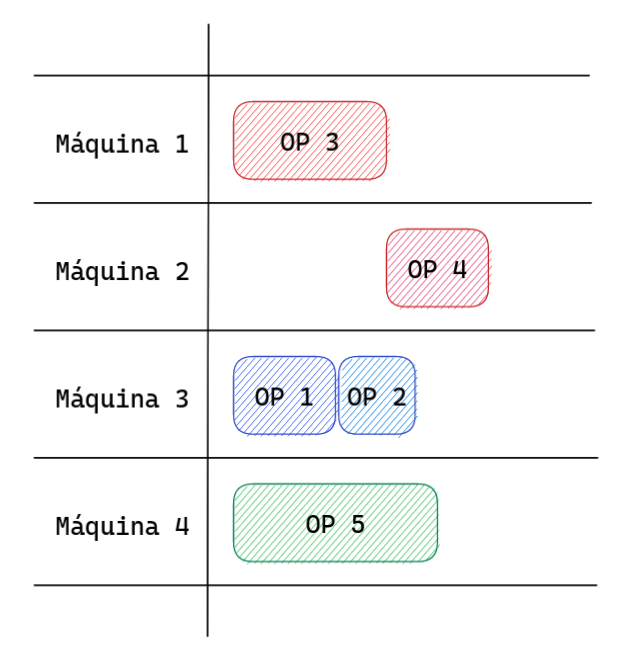
\includegraphics[scale=0.40]{ejemplo.png}
    \caption{Ejemplo de planificación óptima}
    \label{fig:example-solution}
\end{figure}

La distribución final de tiempos para cada máquina es la siguiente: 
\begin{itemize}
    \item \textbf{maquina 1}, OP 3 (3 UT) + 0 GAP = 3 UT 
    \item \textbf{maquina 2}, OP 4 (2 UT) + 3 GAP = 5 UT 
    \item \textbf{maquina 3}, OP 1 (2 UT) + OP 2 (1 UT) + 0 GAP = 3 UT 
    \item \textbf{maquina 4}, OP 5 (4 UT) + 0 GAP = 4 UT. 
\end{itemize}

Ya que el tiempo total de producción es el tiempo de finalización de la máquina más lenta, 
que es la máquina 2, son 5 UT. Notese que el gap de la máquina 2 es deribado de la dependencia
existente entre la operación 4 y la operación 3 por petenercer ambos al trabajo B, 
por lo tanto, antes de que dicha maquina empiece con la operacion 4 tiene que esperar 
a que se procese la máquina 1.

\subsection{Estructura de la memoria}



\pagebreak
    \section{Desarrollo basado en MLOps}
MLOps (Machine Learning Operations) es una extensión de la metodología DevOps (Development Operations)
que se enfoca en la integración, desarrollo y gestión del software de la mano del ciclo de vida del modelo.
Los pilares fundamentales se basan en la automatización y la mejora progresiva de la calidad del modelo,
lo que permite una implementación y puesta en producción mucho más efectiva. Para lograrlo, utiliza herramientas
y técnicas que permiten monitorizar, testear, mejorar y adaptar no solo los modelos sino toda la arquitectura
del sistema de forma continua y escalable. Aquí podemos observar el flujo de información dentro de una
arquitectura MLOps.

\begin{figure}[ht]
    \centering
    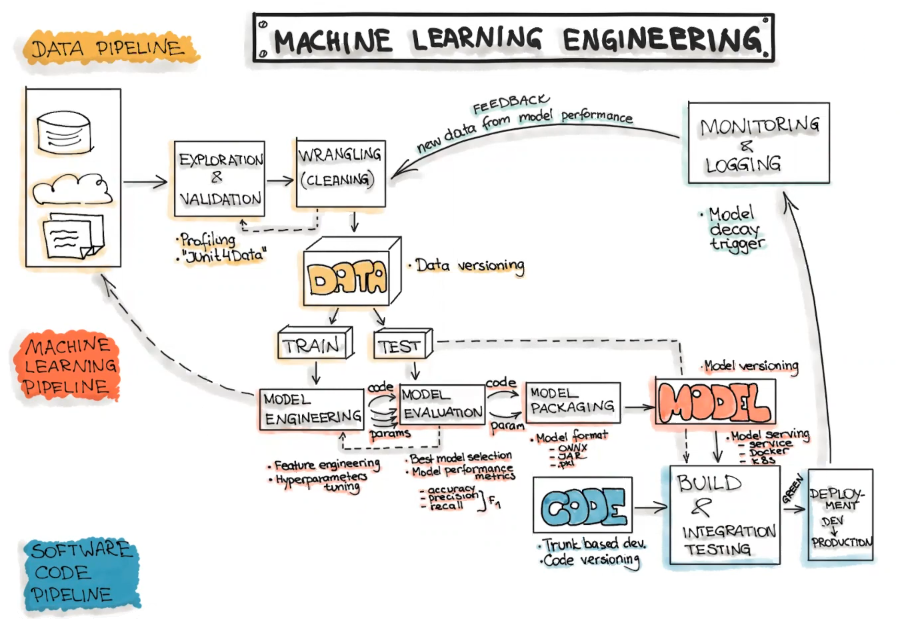
\includegraphics[scale=0.55]{architecture.png}
    \caption{Arquitectura MLOps}
    \label{fig:architecure-mlops}
\end{figure}

\subsection{Principios de MLOps}
A continuación, vamos a detallar los principios de MLOps que vamos a seguir en el desarrollo de nuestro proyecto.
En esta sección se incluyen los puntos más importantes de la metodología, durante todo el desarrollo intentaremos
cumplir con ellos en la medida de lo posible, ya que pueden darse situaciones en las que sea totalmente imposible
satisfacerlos al completo.

\begin{itemize}
    \item \textbf{Automatización}: la automatización es la clave para la eficiencia y la escalabilidad.
          Aqui incluimos tareas como la generación de datos, el despliegue del modelo, la evaluación y
          la puesta en producción.
    \item \textbf{Testeo}: garantiza que tanto la funcionalidad como el desempeño del modelo están evaluados correctamente.
          Esencial en Machine Learning para identificar problemas y mejorar la confianza en los resultados.
    \item \textbf{Versionado}: es importante tener un control de versiones de los datos, el código y los modelos.
          Puede variar el método dependiendo de la herramienta que se utilice, pero existen estándares como Git para la gestión
          de código y GitHub/GitLab para el almacenamiento de los repositorios.
    \item \textbf{Reproducibilidad}: es necesario poder reproducir los resultados de forma consistente, puede ser
          complicado en Machine Learning debido a la naturaleza aleatoria de los algoritmos. Igualmente aquí se trataran
          las herramientas y medidas necesarias para lograrlo.
    \item \textbf{Monitorización}: es importante tener un control de los modelos en proceso de entrenamiento o de producción.
          Por ello, recolectar estadisiticas en tiempo de procesamiento nos ayudará a generar nuevas hipotesis para las proximas interaciones.
\end{itemize}

\subsection{Metodología de trabajo}
Una de las características de los proyectos de Machine Learning es que son tecnologías en constante evolución, el
desarrollo no es un proceso sencillo y requiere de un enfoque coordinado por parte de los diferentes
equipos que lo conforman para asegurar su sostenibilidad a largo plazo. Es fundamental poder adapatarse a los cambios
de forma agil, sin que esto suponga un deterioro del nivel de productividad o que ralentice el avance de nuevas
funcionalidades.\medskip

Podemos identificar tres fases principales: diseño, desarrollo del modelo y operaciones. Cada fase tiene un enfoque
específico y requiere una serie de tareas para garantizar el éxito del proyecto. La fase de diseño,
se definen los objetivos y requisitos del proyecto, se identifican los datos necesarios para el entrenamiento y
se establecen los criterios de éxito. La fase de desarrollo del modelo, se preparan los datos, se entrena el modelo
y se evalúa su rendimiento. También se realiza la validación y se toman las decisiones sobre el modelo final a utilizar.
Finalmente, en la fase de operaciones, se integra el modelo en la infraestructura existente, se monitorea su rendimiento
y se extraen conclusiones para futuras iteraciones. Al repartir las responsabilidades en diferentes fases, aislamos los erroes junto con la carga de trabajo y podemos avanzar
sin la preocuapacion de que un bug o un cambio requisitos afecte al resto del equipo.

\begin{figure}[ht]
    \centering
    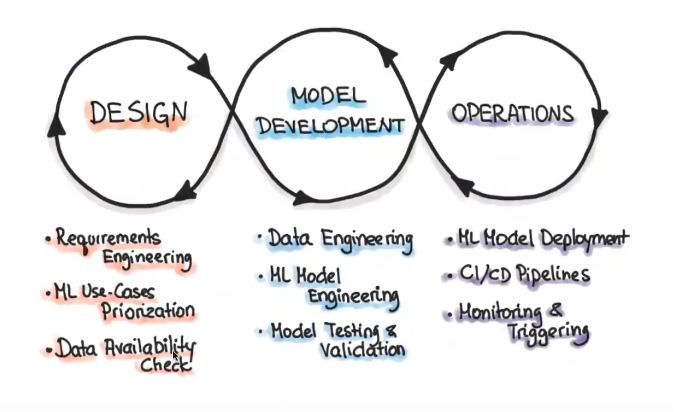
\includegraphics[scale=0.5]{proceso-mlops.png}
    \caption{Metodología MLOps}
    \label{fig:proces-mlops}
\end{figure}

Para visualizar de forma más clara la ventaja que supone este enfoque frente a uno tradicional, a continuación
se mencionara un ejemplos de una posible situacion real. \textbf{Ejemplo:} Tenemos un modelo que actualmente está alojado en AWS y queremos migrarlo a Azure, debido a que
utilizamos MLOps existe configurada una action que en el momento que el equipo publica una nueva release
automáticamente despliega el modelo en el servidor cloud. La parte del equipo encargada de las operaciones procede
a configurar el nuevo servicio y modificar la action para redirigir el despliegue al nuevo servidor. Durante este
tiempo, el equipo de desarrollo a podido avanzar en nuevas mejoras para el modelo y ahora se disponen a volver
a publicar los cambios. Ellos no han notado ningún cambio, pero a nivel de infraestructura se ha realizado una
completa migracion sin afectar en ningún momento en el desarrollo.


\pagebreak
    \section{Herramientas de desarrollo}
    La siguiente sección se enfoca en presentar las herramientas utilizadas para el desarrollo y  
    mantenimiento del codigo fuente del proyecto. Los recursos que se mencionan, si vien ayudan positivamente 
    al ecosistema de trabajo y a la calidad del mismo, es importante destacar que en este apartado no se incluyen 
    detalles sobre ninguna tecnologia directamente relacionada con la implementación del modelo de Machine Learning. 
    Este aspecto se tratará en un apartado posterior del informe.

    \subsection{Jupyter Notebook}

    \subsection{Pyenv y Virtualenv}

    \subsection{Git}

    \subsection{Pip-tools}

    \subsection{Pytest}
    Pytest es una de las mejores opciones para el testing de software y la preferente en proyectos de Python. 
    Es la libreria más popular dentro del Machine Learning debido a su facilidad de uso y  
    permite escribir teses unitarios de forma funcional. Cuenta con una amplia variedad 
    de herramientas para la gestion de pruebas, algunos de sus utilidades más relevantes son las fixtures, que
    optimiza la reutilización de recursos; el mock, que encapsula la funcionalidad de una funcion para poder
    testearla de forma aislada y el coverage, que muestra que zonas del codigo están cubiertas por la suit de teses. 

    \subsection{Pre-commit}

    \subsection{Makefile}

    \subsection{Flake8}

    \subsection{Black}
    
    \subsection{Docker}
    

\pagebreak
    \section{Sistema de evaluación del modelo}
    Un buen sistema de evaluación es esencial para un proyecto de machine learning. 
    No solo es útil por el hecho de medir la precisión y el rendimiento de los modelos, 
    sino que además sirve como un identificador claro de nuestro progeso dentro del desarrollo. 
    El seleccionar el modelo óptimo en fases tempranas del proceso no es tan importante 
    como el saber que las iteraciones en las que gastamos tiempo y recursos estan teniendo un impacto 
    positivo en su aprendizaje. Aunque físicamente es imposible conseguir una productividad 
    perfecta, con ayuda de una metodología sólida es posible reducir al maximo esta problemática.
    
    \subsection{Selección de métrica}
    El objetivo de una métrica es, mediante ponderacion numérica, identificar errores en el modelo y 
    servir como ayuda para la toma de decisiones, cambios en el diseñe o la soluación de problemas. En el caso del 
    FJSP, el objetivo es encontrar una acorde a la tarea que queramos abordar. En la literatura se atacan dos puntos
    principalmente: \textit{minimizar el tiempo de finalización} y \textit{minimizar el tiempo de espera entre máquinas}. 

    \begin{itemize}
        \item \textbf{Minimizar el tiempo de espera entre máquinas:} mide el tiempo promedio que cada operación debe 
        esperar antes de ser procesado en una máquina específica. Esta métrica es importante porque 
        indica la eficiencia del sistema en términos de cómo se están utilizando los recursos disponibles 
        y cómo se gestionan los trabajos en las colas.
        \item \textbf{Minimizar el tiempo de finalización:} se basa en el tiempo total que se tarda en completar todos 
        los trabajos del sistema. Es un buen indicador porque evalúa el rendimiento global del sistema 
        y la eficacia para completar el proceso en el plazo establecido. 
    \end{itemize}

    Aunque ambas métricas son importantes, la segunda es la que se vamos a utilizar como referencia en cuanto al
    desempeño del modelo, ya que uno de nuestros objetivos principales es reducir los tiempos de producción y no tanto
    aprobechar las máquinas lo máximo posible. Es posible utilizar ambas para identificar puntos débiles tanto del modelo 
    como del propio proceso que se quiere optimizar pero, por la propia idiosincrasia de las mismas, el mejorar la puntuación
    en una de ellas inevitablemente afectara negativamente la puntuación de la otra en un amplio número de casuísticas.

    \subsection{Implementación de la métrica} 


\pagebreak

    \printbibliography[title=Bibliografía]

\end{document}